\documentclass[12pt,titlepage]{article}
\usepackage[margin=1.25in]{geometry}
\usepackage{graphicx,amsmath,minted}

%% Variables definition
\newcommand{\vSubject}{Advanced Database}
\newcommand{\vSubtitle}{Window, Ranking, Offset, and Aggregate}
\newcommand{\vName}{Dicha Zelianivan Arkana}
\newcommand{\vNIM}{2241720002}
\newcommand{\vClass}{2i}
\newcommand{\vDepartment}{Information Technology}
\newcommand{\vStudyProgram}{D4 Informatics Engineering}

%% [START] Tikz related stuff
\usepackage{tikz}
\usetikzlibrary{svg.path,calc,shapes.geometric,shapes.misc}
\tikzstyle{terminator} = [rectangle, draw, text centered, rounded corners = 1em, minimum height=2em]
\tikzstyle{preparation} = [chamfered rectangle, chamfered rectangle sep=0.75em, draw, text centered, minimum height = 2em]
\tikzstyle{process} = [rectangle, draw, text centered, minimum height=2em]
\tikzstyle{decision} = [diamond, aspect=2, draw, text centered, minimum height=2em]
\tikzstyle{data}=[trapezium, draw, text centered, trapezium left angle=60, trapezium right angle=120, minimum height=2em]
\tikzstyle{connector} = [line width=0.25mm,->]
%% [END] Tikz related stuff

%% [START] Fancy header related stuff
\usepackage{fancyhdr}
\pagestyle{fancy}
\setlength{\headheight}{15pt} % compensate fancyhdr style
\fancyhead{}
\fancyfoot{}
\fancyfoot[L]{\thepage}
\fancyfoot[R]{\textit{\vSubject - \vSubtitle}}
\renewcommand{\footrulewidth}{0.4pt}% default is 0pt, overline for footer
%% [END] Fancy header related stuff

%% [START] Custom tabular command related stuff
\usepackage{tabularx}
\newcommand{\details}[2]{
    #1 & #2  \\
}
%% [END] Custom tabular command related stuff

%% [START] Figure related stuff
\newcommand{\image}[3][1]{
    \begin{figure}[h]
        \centering
        \includegraphics[#1]{#2}
        \caption{#3}
        \label{#3}
    \end{figure}
}
%% [END] Figure related stuff

\begin{document}
\begin{titlepage}
    \centering
    \vfill
    {\bfseries\LARGE
        \vSubject\\
        \vskip0.25cm
        \vSubtitle
    }
    \vfill
    
\includegraphics[width=6cm]{images/polinema-logo.png}
    \vfill
    {
        \textbf{Name}\\
        \vName\\
        \vskip0.5cm
        \textbf{NIM}\\
        \vNIM\\
        \vskip0.5cm
        \textbf{Class}\\
        \vClass\\
        \vskip0.5cm
        \textbf{Department}\\
        \vDepartment\\
        \vskip0.5cm
        \textbf{Study Program}\\
        \vStudyProgram
    }
\end{titlepage}

\section{Practicum}
\begin{enumerate}
    \item {
        Tulislah pernyataan \texttt{SELECT} untuk mengambil kolom \texttt{orderid}, \texttt{orderdate}, dan \texttt{val} serta
        kolom hasil perhitungan bernama \texttt{rowno} dari view \texttt{Sales.OrderValues}! Gunakan fungsi
        \texttt{ROW\_NUMBER} untuk mengembalikan \texttt{rowno}, urutkan nomor baris berdasarkan kolom
        orderdate!
        
        \begin{minted}[autogobble,fontsize=\small]{sql}
            SELECT
                orderid,
                orderdate,
                val,
                rowno = ROW_NUMBER() OVER (ORDER BY orderdate)
            FROM
                Sales.OrderValues;
        \end{minted}

        \begin{center}
            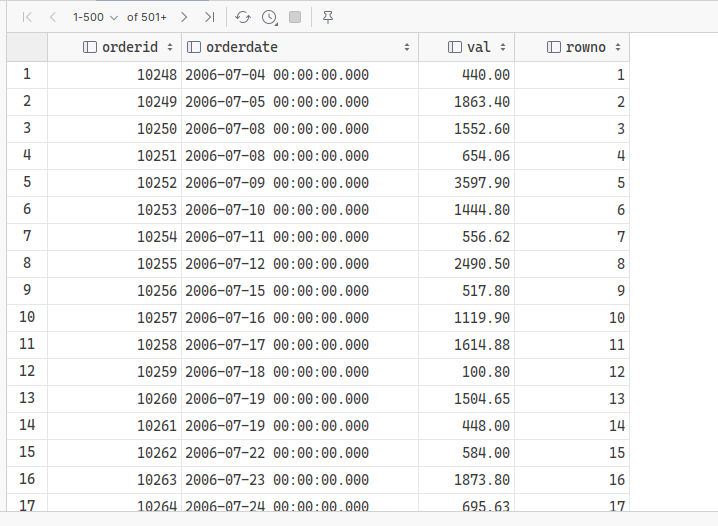
\includegraphics[width=.8\textwidth]{./images/1.png}
        \end{center}
    }
    \pagebreak
    \item {
        Salin T-SQL pada soal no 1. Kemudian modifikasi dengan memasukkan kolom tambahan
        bernama rankno. Untuk membuat rankno gunakan fungsi RANK dengan urutan peringkat
        berdasarkan kolom orderdate!

        \begin{minted}[autogobble,fontsize=\small]{sql}
            SELECT
                orderid,
                orderdate,
                val,
                rowno = ROW_NUMBER() OVER (ORDER BY orderdate),
                rankno = RANK() OVER (ORDER BY orderdate)
            FROM
                Sales.OrderValues;
        \end{minted}
    
        \begin{center}
            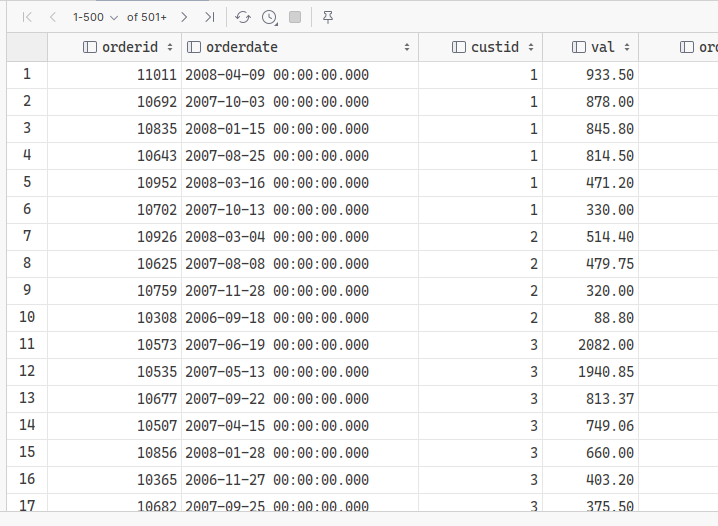
\includegraphics[width=.8\textwidth]{./images/2.png}
        \end{center}
    }
    \item {
        Apakah perbedaan antara fungsi \texttt{RANK} dan fungsi \texttt{ROW\_NUMBER}?

        \begin{itemize}
            \item {
                \texttt{ROW\_NUMBER} akan mengembalikan nomor baris yang unik untuk setiap baris dalam partisi.
            }
            \item {
                \texttt{RANK} akan mengembalikan peringkat baris dalam partisi dengan nilai yang sama. Nilai peringkat tidak akan berurutan jika ada nilai yang sama.
            }
        \end{itemize}
    }
    \pagebreak
    \item {
        Tuliskan pernyataan \texttt{SELECT} untuk mengambil kolom \texttt{orderid}, \texttt{orderdate}, \texttt{custid}, dan \texttt{val}
        serta hitung kolom bernama {orderrankno} dari view \texttt{Sales.OrderValues}. Kolom \texttt{orderrankno}
        harus menampilkan rangking per pelanggan secara independen, berdasarkan pemesanan val
        dalam urutan menurun!

        \begin{minted}[autogobble,fontsize=\small]{sql}
            SELECT
                orderid,
                orderdate,
                custid,
                val,
                orderrankno = RANK() OVER (PARTITION BY custid ORDER BY val DESC)
            FROM
                Sales.OrderValues;
        \end{minted}

        \begin{center}
            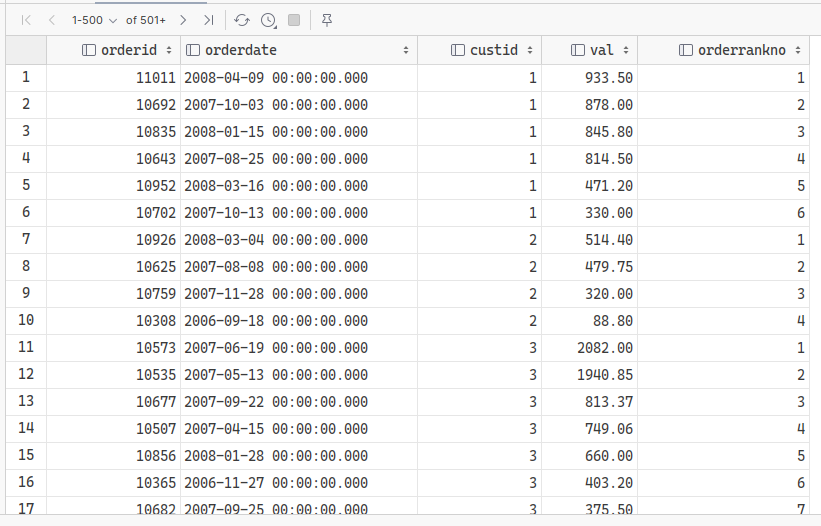
\includegraphics[width=.8\textwidth]{./images/4.png}
        \end{center}
    }
    \pagebreak
    \item {
        Tuliskan pernyataan \texttt{SELECT} untuk mengambil kolom custid dan val dari view
        \texttt{Sales.OrderValues}. Tambahkan dua kolom berikut:
        1) \texttt{orderyear} sebagai tahun dari kolom orderdate
        2) \texttt{orderrankno} sebagai nomor urut, dipartisi berdasarkan pelanggan dan tahun pesanan,
        dan diurutkan berdasarkan nilai pesanan dalam urutan menurun!

        \begin{minted}[autogobble,fontsize=\small]{sql}
            SELECT
                custid,
                val,
                orderyear = YEAR(orderdate),
                orderrankno = RANK() OVER (PARTITION BY custid, 
                                           YEAR(orderdate) ORDER BY val DESC)
            FROM
                Sales.OrderValues;
        \end{minted}

        \begin{center}
            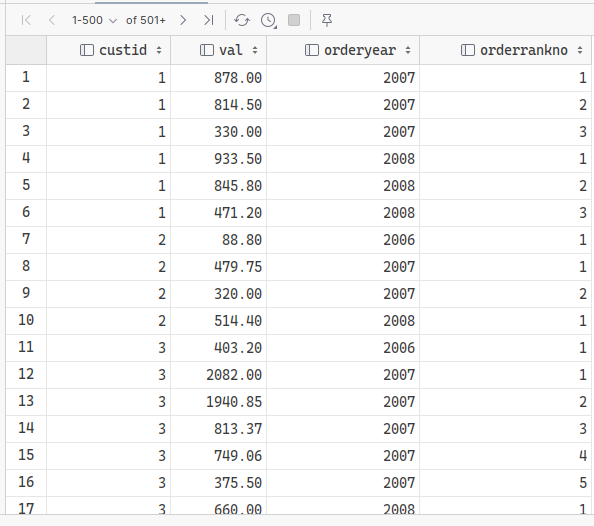
\includegraphics[width=.8\textwidth]{./images/5.png}
        \end{center}
    }
    \pagebreak
    \item {
        Salin query jawaban soal nomor 6 dan modifikasi untuk memfilter hanya pesanan
        dengan dua peringkat paling awal berdasarkan kolom orderrankno!

        \begin{minted}[autogobble,fontsize=\small]{sql}
            WITH RankedOrderValues AS (
                SELECT custid,
                    val,
                    orderyear   = YEAR(orderdate),
                    orderrankno = RANK() OVER (PARTITION BY custid,
                        YEAR(orderdate) ORDER BY val DESC)
                FROM Sales.OrderValues
            )
            SELECT custid, orderyear, orderrankno, val
            FROM RankedOrderValues
            WHERE orderrankno <= 2
        \end{minted}

        \begin{center}
            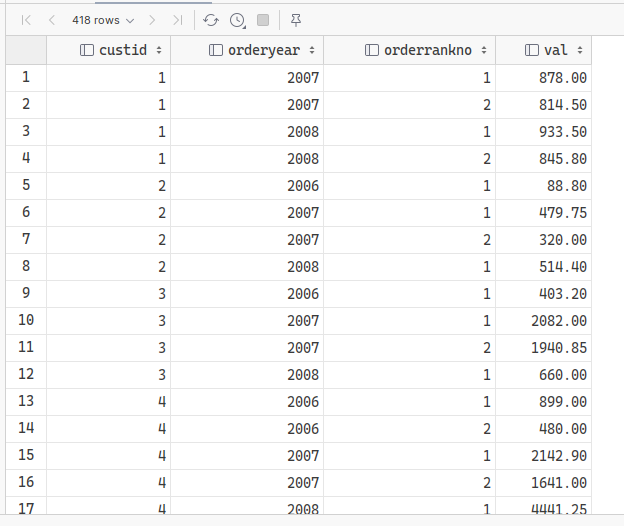
\includegraphics[width=.8\textwidth]{./images/6.png}
        \end{center}
    }
    \pagebreak
    \item {
        Buatlah (common table expression) CTE dengan nama OrderRows berdasarkan query yang
        mengambil kolom \texttt{orderid}, \texttt{orderdate}, and \texttt{val} dari view \texttt{Sales.OrderValues}. Tambahkan kolom
        hasil perhitungan dengan nama {rowno} menggunakan fungsi \texttt{ROW\_NUMBER} yang diurutkan
        berdasarkan kolom \texttt{orderdate} dan \texttt{orderid}!

        \begin{minted}[autogobble,fontsize=\small]{sql}
            WITH OrderRows AS (
                SELECT
                    orderid,
                    orderdate,
                    val,
                    rowno = ROW_NUMBER() OVER (ORDER BY orderdate, orderid)
                FROM
                    Sales.OrderValues
            )
            SELECT * FROM OrderRows;
        \end{minted}

        \begin{center}
            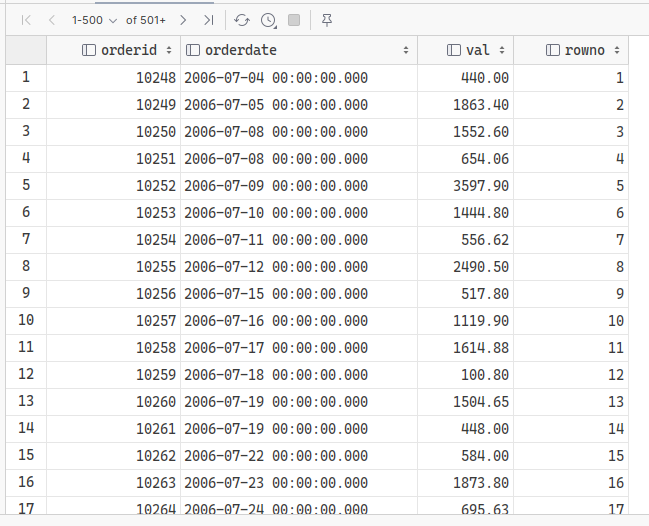
\includegraphics[width=.8\textwidth]{./images/7.png}
        \end{center}
    }
    \pagebreak
    \item {
        Tuliskan pernyataan SELECT terhadap CTE dan gunakan \texttt{LEFT JOIN} dengan CTE yang sama
        untuk mengambil baris saat ini (current row) dan baris sebelumnya (previous row) berdasarkan
        kolom rowno. Kembalikan kolom \texttt{orderid}, \texttt{orderdate}, and \texttt{val} untuk baris saat ini dan kolom val
        untuk baris sebelumnya sebagai \texttt{prevval}. Tambahkan kolom hasil perhitungan dengan nama
        \texttt{diffprev} yang menunjukkan perbedaan antara val saat ini dengan sebelumnya!

        \begin{minted}[autogobble,fontsize=\small]{sql}
            WITH OrderRows AS (
                SELECT
                    orderid,
                    orderdate,
                    val,
                    rowno = ROW_NUMBER() OVER (ORDER BY orderdate, orderid)
                FROM
                    Sales.OrderValues
            )
            SELECT
                curr.orderid,
                curr.orderdate,
                curr.val,
                prev.val AS prevval,
                diffprev = curr.val - prev.val
            FROM
                OrderRows curr
                LEFT JOIN OrderRows prev ON curr.rowno = prev.rowno + 1;
        \end{minted}

        \begin{center}
            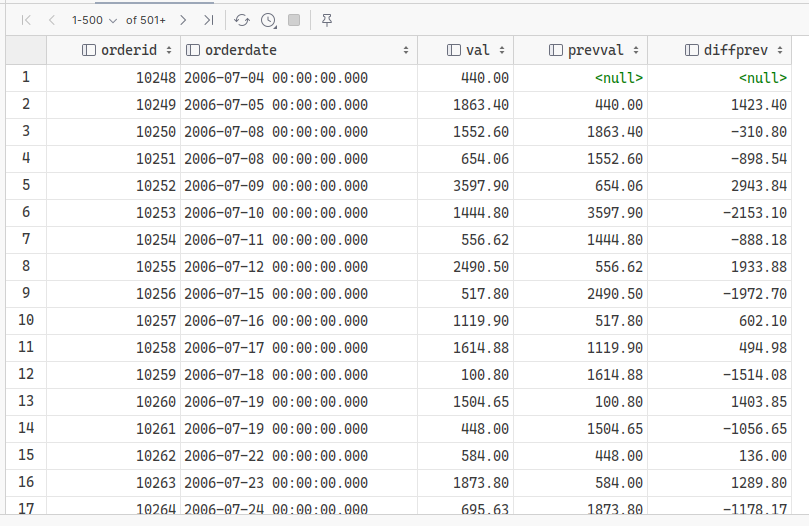
\includegraphics[width=.8\textwidth]{./images/8.png}
        \end{center}
    }
    \pagebreak
    \item {
        Tuliskan pernyataan \texttt{SELECT} menggunakan fungsi LAG untuk mendapat hasil yang sama
        dengan query pada soal no.2! Query tidak yang dibuat pada soal ini tidak menggunakan CTE.

        \begin{minted}[autogobble,fontsize=\small]{sql}
            SELECT
                orderid,
                orderdate,
                val,
                prevval = LAG(val, 1, 0) OVER (ORDER BY orderdate),
                diffprev = val - LAG(val, 1, 0) OVER (ORDER BY orderdate)
            FROM
                Sales.OrderValues;
        \end{minted}

        \begin{center}
            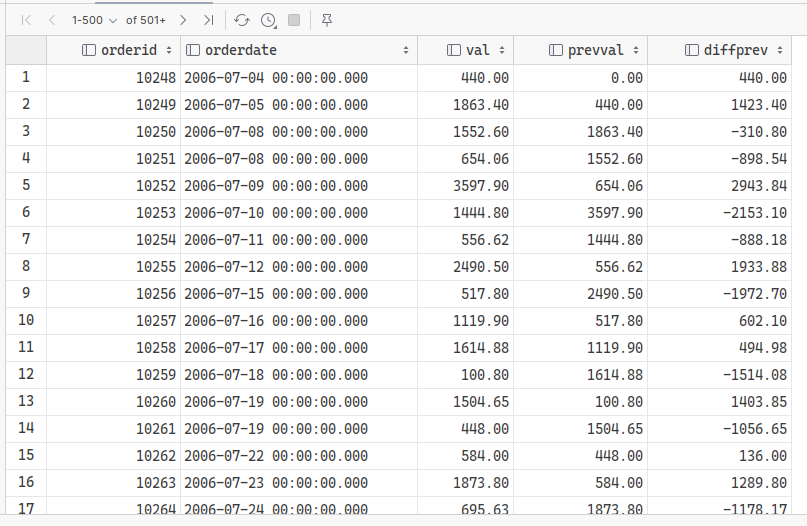
\includegraphics[width=.8\textwidth]{./images/9.png}
        \end{center}
    }
    \pagebreak
    \item {
        Buatlah sebuah CTE bernama \texttt{SalesMonth2007} yang membuat dua kolom yaitu,
        \texttt{monthno} (jumlah bulan dari kolom \texttt{orderdate}) dan \texttt{val} (agregat dari kolom \texttt{val})! Kemudian filter
        hasilnya hanya untuk tahun pesanan 2007 dan dikelompokkan berdasarkan \texttt{monthno}!

        \begin{minted}[autogobble,fontsize=\small]{sql}
            WITH SalesMonth2007 AS (
                SELECT
                    monthno = MONTH(orderdate),
                    val = SUM(val)
                FROM
                    Sales.OrderValues
                WHERE
                    YEAR(orderdate) = 2007
                GROUP BY
                    MONTH(orderdate)
            )
            SELECT * FROM SalesMonth2007;
        \end{minted}

        \begin{center}
            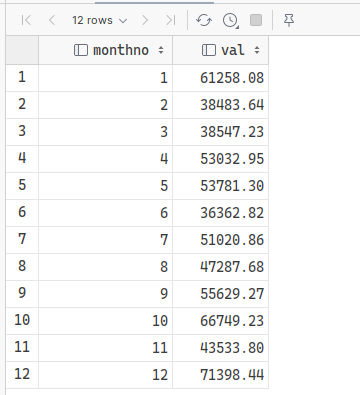
\includegraphics[width=.5\textwidth]{./images/10.png}
        \end{center}
    }
    \pagebreak
    \item {
        Tuliskan pernyataan \texttt{SELECT} yang akan mengambil kolom \texttt{monthno} dan \texttt{val} dari CTE
        dan tambahkan 3 kolom untuk ditampilkan, yaitu :
        \begin{enumerate}
            \item \texttt{avglast3months} (jumlah penjualan rata-rata tiga bulan terakhir)
            \item \texttt{diffjanuary} (perbedaan antara val saat ini dengan val pada bulan januari, gunakan fungsi \texttt{FIRST\_VALUE})
            \item \texttt{nextval} (nilai dari kolom val pada bulan selanjutnya)
        \end{enumerate}
        \small
        Informasi : Jumlah rata-rata untuk tiga bulan terakhir tidak dihitung dengan benar karena jumlah
        total 2 bulan pertama dibagi dengan 3.

        \begin{minted}[autogobble,fontsize=\small]{sql}
            WITH SalesMonth2007 AS (
                SELECT
                    monthno = MONTH(orderdate),
                    val = SUM(val)
                FROM
                    Sales.OrderValues
                WHERE
                        YEAR(orderdate) = 2007
                GROUP BY
                    MONTH(orderdate)
            )
            SELECT
                monthno,
                val,
                avglast3months = ISNULL(AVG(val) OVER (ORDER BY monthno ROWS 
                                                       BETWEEN 3 PRECEDING AND 1 PRECEDING), 0),
                diffjanuary = val - FIRST_VALUE(val) OVER (ORDER BY monthno),
                nextval = LEAD(val, 1, 0) OVER (ORDER BY monthno)
            FROM
                SalesMonth2007;
        \end{minted}

        \begin{center}
            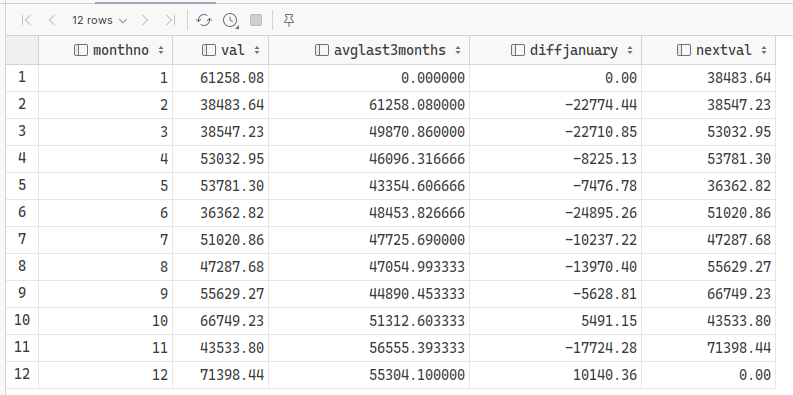
\includegraphics[width=.8\textwidth]{./images/11.png}
        \end{center}
    }
    \pagebreak
    \item {
        Tuliskan pernyataan \texttt{SELECT} untuk mengambil kolom \texttt{custid}, \texttt{orderid}, \texttt{orderdate}, dan
        \texttt{val} dari view \texttt{Sales.OrderValues}. Tambahkan kolom bernama {percoftotalcust} yang berisi
        persentase nilai masing-masing jumlah pesanan penjualan dibandingkan dengan jumlah
        penjualan untuk pelanggan tersebut!

        \begin{minted}[autogobble,fontsize=\small]{sql}
            SELECT
                custid,
                orderid,
                orderdate,
                val,
                percoftotalcust = val / SUM(val) OVER (PARTITION BY custid)
            FROM
                Sales.OrderValues;
        \end{minted}

        \begin{center}
            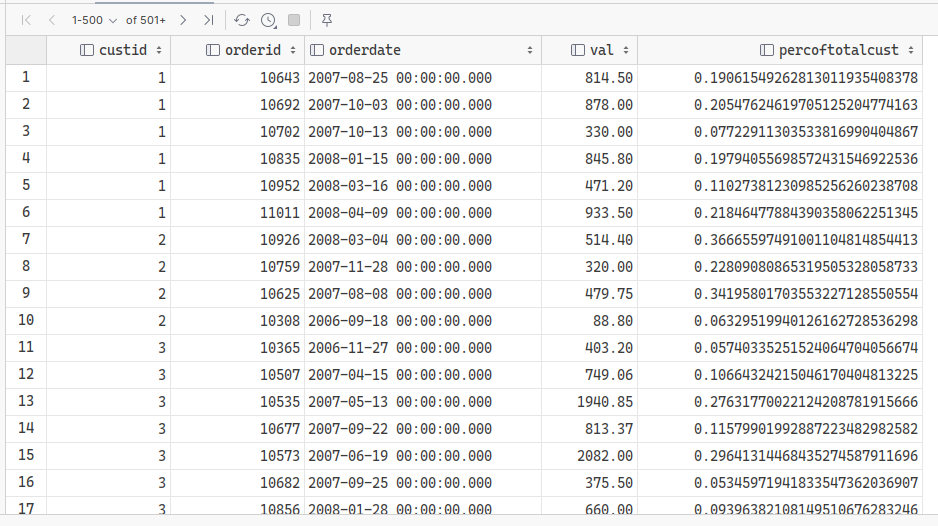
\includegraphics[width=.8\textwidth]{./images/12.png}
        \end{center}
    }
    \pagebreak
    \item {
        Salin pernyataan \texttt{SELECT} sebelumnya dan modifikasi dengan menambahkan kolom
        yang baru dihitung bernama \texttt{runval}! Kolom ini harus berisi total penjualan yang sedang terjadi
        untuk setiap pelanggan berdasarkan tanggal pemesanan, menggunakan \texttt{orderid} sebagai
        tiebreaker.

        \begin{minted}[autogobble,fontsize=\small]{sql}
            SELECT
                custid,
                orderid,
                orderdate,
                val,
                percoftotalcust = val / SUM(val) OVER (PARTITION BY custid),
                runval = SUM(val) OVER (PARTITION BY custid ORDER BY orderdate, orderid)
            FROM
                Sales.OrderValues;
        \end{minted}

        \begin{center}
            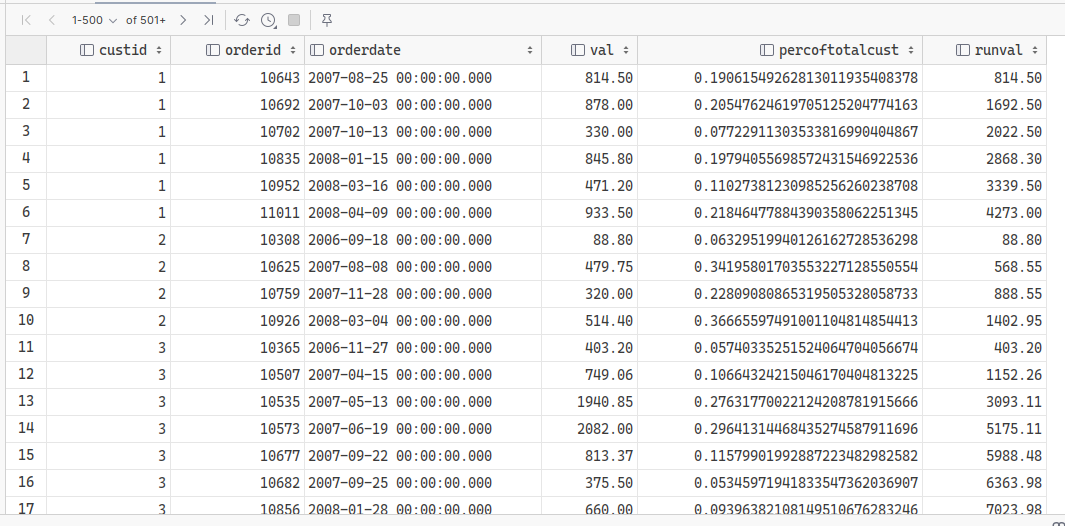
\includegraphics[width=.8\textwidth]{./images/13.png}
        \end{center}
    }
    \pagebreak
    \item {
        Salin CTE SalesMonth2007 dalam percobaan 2. Tuliskan pernyataan SELECT untuk
        mengambil kolom monthno dan val. Tambahkan dua kolom yang dihitung:

        \begin{enumerate}
            \item \texttt{avglast3months}. Kolom ini harus berisi jumlah penjualan rata-rata untuk tiga bulan
            terakhir sebelum bulan saat ini menggunakan fungsi window agregat. Asumsikan bahwa tidak ada missing months.
            \item \texttt{ytdval} Kolom ini harus berisi nilai penjualan kumulatif sampai dengan bulan saat ini.
        \end{enumerate}

        \begin{minted}[autogobble,fontsize=\small]{sql}
            WITH SalesMonth2007 AS (
                SELECT
                    monthno = MONTH(orderdate),
                    val = SUM(val)
                FROM
                    Sales.OrderValues
                WHERE
                    YEAR(orderdate) = 2007
                GROUP BY
                    MONTH(orderdate)
            )
            SELECT
                monthno,
                val,
                avglast3months = ISNULL(AVG(val) OVER (ORDER BY monthno ROWS 
                                                       BETWEEN 3 PRECEDING AND 1 PRECEDING), 0),
                ytdval = SUM(val) OVER (ORDER BY monthno)
            FROM
                SalesMonth2007;
        \end{minted}

        \begin{center}
            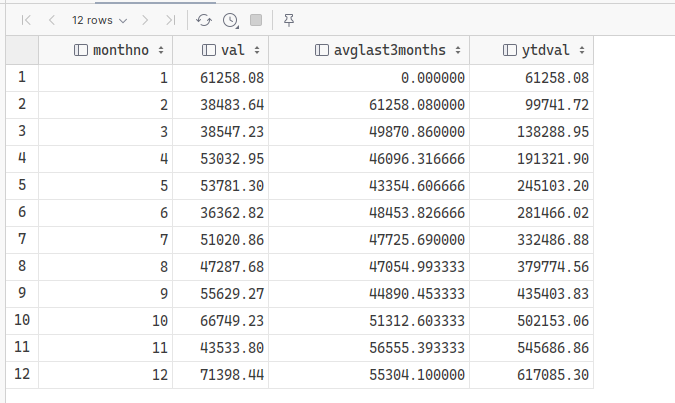
\includegraphics[width=.8\textwidth]{./images/14.png}
        \end{center}
    }
\end{enumerate}


\end{document}

